\documentclass[12pt,a4paper]{article}
\usepackage[polish]{babel}
\usepackage[T1]{fontenc}
\usepackage[utf8x]{inputenc}
\usepackage{hyperref}
\usepackage{url}
\usepackage[]{algorithm2e}
\usepackage{listings}
\usepackage{graphicx}
\usepackage{color}
\usepackage{listings}
\usepackage{fancyhdr}
\usepackage{pgfplots}
\usepackage{pgf-pie} 
\usepackage{newtxtext,newtxmath}
\usepackage{float}
\usepackage{amsmath}
\usepackage{caption}
\usepackage{multirow}
\usepackage{colortbl}
\usepackage{hhline}

\pgfplotsset{compat=1.18}

\lstloadlanguages{% Check Dokumentation for further languages ...
	C,
	C++,
	csh,
	Java
}

\definecolor{red}{rgb}{0.6,0,0} % for strings
\definecolor{blue}{rgb}{0,0,0.6}
\definecolor{green}{rgb}{0,0.8,0}
\definecolor{cyan}{rgb}{0.0,0.6,0.6}

\newtheorem{twr}{Twierdzenie}

\lstset{
	language=csh,
	basicstyle=\footnotesize\ttfamily,
	numbers=left,
	numberstyle=\tiny,
	numbersep=5pt,
	tabsize=2,
	extendedchars=true,
	breaklines=true,
	frame=b,
	stringstyle=\color{blue}\ttfamily,
	showspaces=false,
	showtabs=false,
	xleftmargin=17pt,
	framexleftmargin=17pt,
	framexrightmargin=5pt,
	framexbottommargin=4pt,
	commentstyle=\color{green},
	morecomment=[l]{//}, %use comment-line-style!
	morecomment=[s]{/*}{*/}, %for multiline comments
	showstringspaces=false,
	morekeywords={ abstract, event, new, struct,
		as, explicit, null, switch,
		base, extern, object, this,
		bool, false, operator, throw,
		break, finally, out, true,
		byte, fixed, override, try,
		case, float, params, typeof,
		catch, for, private, uint,
		char, foreach, protected, ulong,
		checked, goto, public, unchecked,
		class, if, readonly, unsafe,
		const, implicit, ref, ushort,
		continue, in, return, using,
		decimal, int, sbyte, virtual,
		default, interface, sealed, volatile,
		delegate, internal, short, void,
		do, is, sizeof, while,
		double, lock, stackalloc,
		else, long, static,
		enum, namespace, string},
	keywordstyle=\color{cyan},
	identifierstyle=\color{red},
}

\usepackage{caption}
\DeclareCaptionFont{white}{\color{white}}
\DeclareCaptionFormat{listing}{\colorbox{blue}{\parbox{\textwidth}{\hspace{15pt}#1#2#3}}}
\captionsetup[lstlisting]{format=listing,labelfont=white,textfont=white, singlelinecheck=false, margin=0pt, font={bf,footnotesize}}


\addtolength{\hoffset}{-1.5cm}
\addtolength{\marginparwidth}{-1.5cm}
\addtolength{\textwidth}{3cm}
\addtolength{\voffset}{-1cm}
\addtolength{\textheight}{2.5cm}
\setlength{\topmargin}{0cm}
\setlength{\headheight}{0cm}

\newcommand\blankpage{%
    \null
    \thispagestyle{empty}%
    \addtocounter{page}{-1}%
    \newpage}

\begin{document}

    \pagestyle{fancy}
    \rhead{\textit{Bazy danych} - Projekt systemu przechowywania danych dla sklepu}

    \title{
    \vspace*{3cm}
    \textbf{Projekt systemu przechowywania danych dla sklepu}}
    \author{Adam Paździerz\\ Dawid Wydra\\ Jakub Gurgul\\ Mariusz Pyrk\\ 
            \vspace*{0.5cm} \\      
            Bazy Danych\\
            \textit{Informatyka - profil praktyczny}\\
            Wydział Matematyki Stosowanej\\
            \textbf{Politechnika Śląska}\\
            Gliwice, Polska
    }
    \date{\today}
	
	\maketitle
	\newpage

    \tableofcontents
    \thispagestyle{empty}
    \newpage

	\section{Wstęp}

        \subsection{Cel}
            Celem projektu jest zaplanowanie oraz wykonanie bazy danych dla średniej wielkości sieci sklepów. Program przeznaczony jest dla pracowników oraz klientów sklepu. Pomoże nadzorować pracę firmy w wielu jej aspektach: dostawy, dystrybucja produktów, zarządzanie umowami, logowanie pracowników oraz klientów.
            
        \subsection{Podział zadań}
            \begin{enumerate}
                \item \textbf{Adam Paździerz} - stworzenie związków encji, związków binarnych oraz modelu relacyjnego;
                \item \textbf{Dawid Wydra} - stworzenie modelu relacyjnego;
                \item \textbf{Jakub Gurgul} - tworzenie dokumentacji, wdrożenie projektu bazy;
                \item \textbf{Mariusz Pyrk} - wdrożenie projektu bazy.
            \end{enumerate}

        \subsection{Założenia}
            Przed przystąpieniem do wykonania, przemyślano jakie cele powinna spełniać baza danych dla sieci sklepów, tak aby móc jak najefektywniej spełniać swoje zadanie. Podstawowe założenia to możliwość logowania użytkowników oraz pozyskiwanie informacji o poniższych aspektach firmy:
            \begin{enumerate}
                \item \textbf{Pracownicy} - obsługa pensji, podpisanych umów, przydzielonego stanowiska, danych personalnych oraz poświadczeń bezpieczeństwa;
                \item \textbf{Sklepy} - identyfikacja pracowników przypisanych do placówki, sprawdzenie stanu magazynowego oraz obsługiwanych zamówień;
                \item \textbf{Klienci} - dane kontaktowe oraz adres do dostawy, złożone zamówienia;
                \item \textbf{Zamówienia} - sumaryczna kwota, zamówione produkty, pracownik oraz sklep obsługujący;
                \item \textbf{Produkty} - ilość sztuk na stanie, przypisane dostawy oraz cena jednostkowa;
                \item \textbf{Dostawcy} - spis oraz artykuły które dostarczają;
                \item Baza będzie pozwalała na zalogowanie się pracownika do systemu, i zgodnie z swoim stanowiskiem na przejrzenie aktywnych zleceń, sprawdzenie stanu magazynowego sklepu, swoich umów, umów sklepu lub całej sieci, sprawdzić oraz dodać nowych pracowników, klientów i dostawców;
                \item Przewidujemy trzy poziomy dostępu dla pracowników: sprzedawca, kierownik sklepu oraz kierownik regionalny; 
                \item Klient będzie mógł zalogować się, podejrzeć jakie zamówienia złożył oraz zamówić nowe.
            \end{enumerate}
            
        \subsection{Encje}
            \begin{enumerate}
                \item \textbf{Pracownik\_uwierzytelnienie} - ID[PK], Login, Hasło, Hasło\_Ostatnia\_Zmiana, UUID, RFID;
                \item \textbf{Pracownicy} - ID[PK], Imię, Nazwisko, Miasto, Adres, Telefon, E-mail, PESEL;
                \item \textbf{Sklepy} - ID[PK], Miasto, Adres, Telefon, E-mail;
                \item \textbf{Klienci} - ID[PK], Imię, Nazwisko, Czy\_firma, Nazwa\_firma, NIP, Miasto, Adres, Telefon, E-mail, Hasła, Hasło\_ostatnia\_zmiana;
                \item \textbf{Produkty} - ID[PK], Nazwa, Kategoria, Opis, Cena, Uwagi.
                \item \textbf{Dostawcy} - ID[PK], Nazwa, Miasto, Adres, Telefon, E-mail, NIP, Uwagi.
            \end{enumerate}
            
        \subsection{Związki}
            \begin{enumerate}
                \item \textbf{Logowanie} - (Pracownicy - Pracownik\_uwierzytelnienie) - 1:1
                \item \textbf{Obsługa zamówień} - (Pracownicy, Klienci, Produkty, Sklepy) - n:n:n:n \newline
                Atrybuty: Data zamówienia, Ilość 
                \item \textbf{Podpisywanie umowy} - (Pracownicy, Sklepy) - n:n \newline
                Atrybuty: Wypłata, Numer umowy, Data Podpisania, Data Zakończenia
                \item \textbf{Dostarczanie produktów} - (Dostawcy, Produkty) - 1:n \newline
                Atrybuty: Ilość, Cena
                \item \textbf{Magazynowanie} - (Sklep, Produkty) - n:n \newline
                Atrybuty: Ilość
            \end{enumerate}

    \section{Diagram związków encji} 
        \begin{figure}[H]
            \centering
            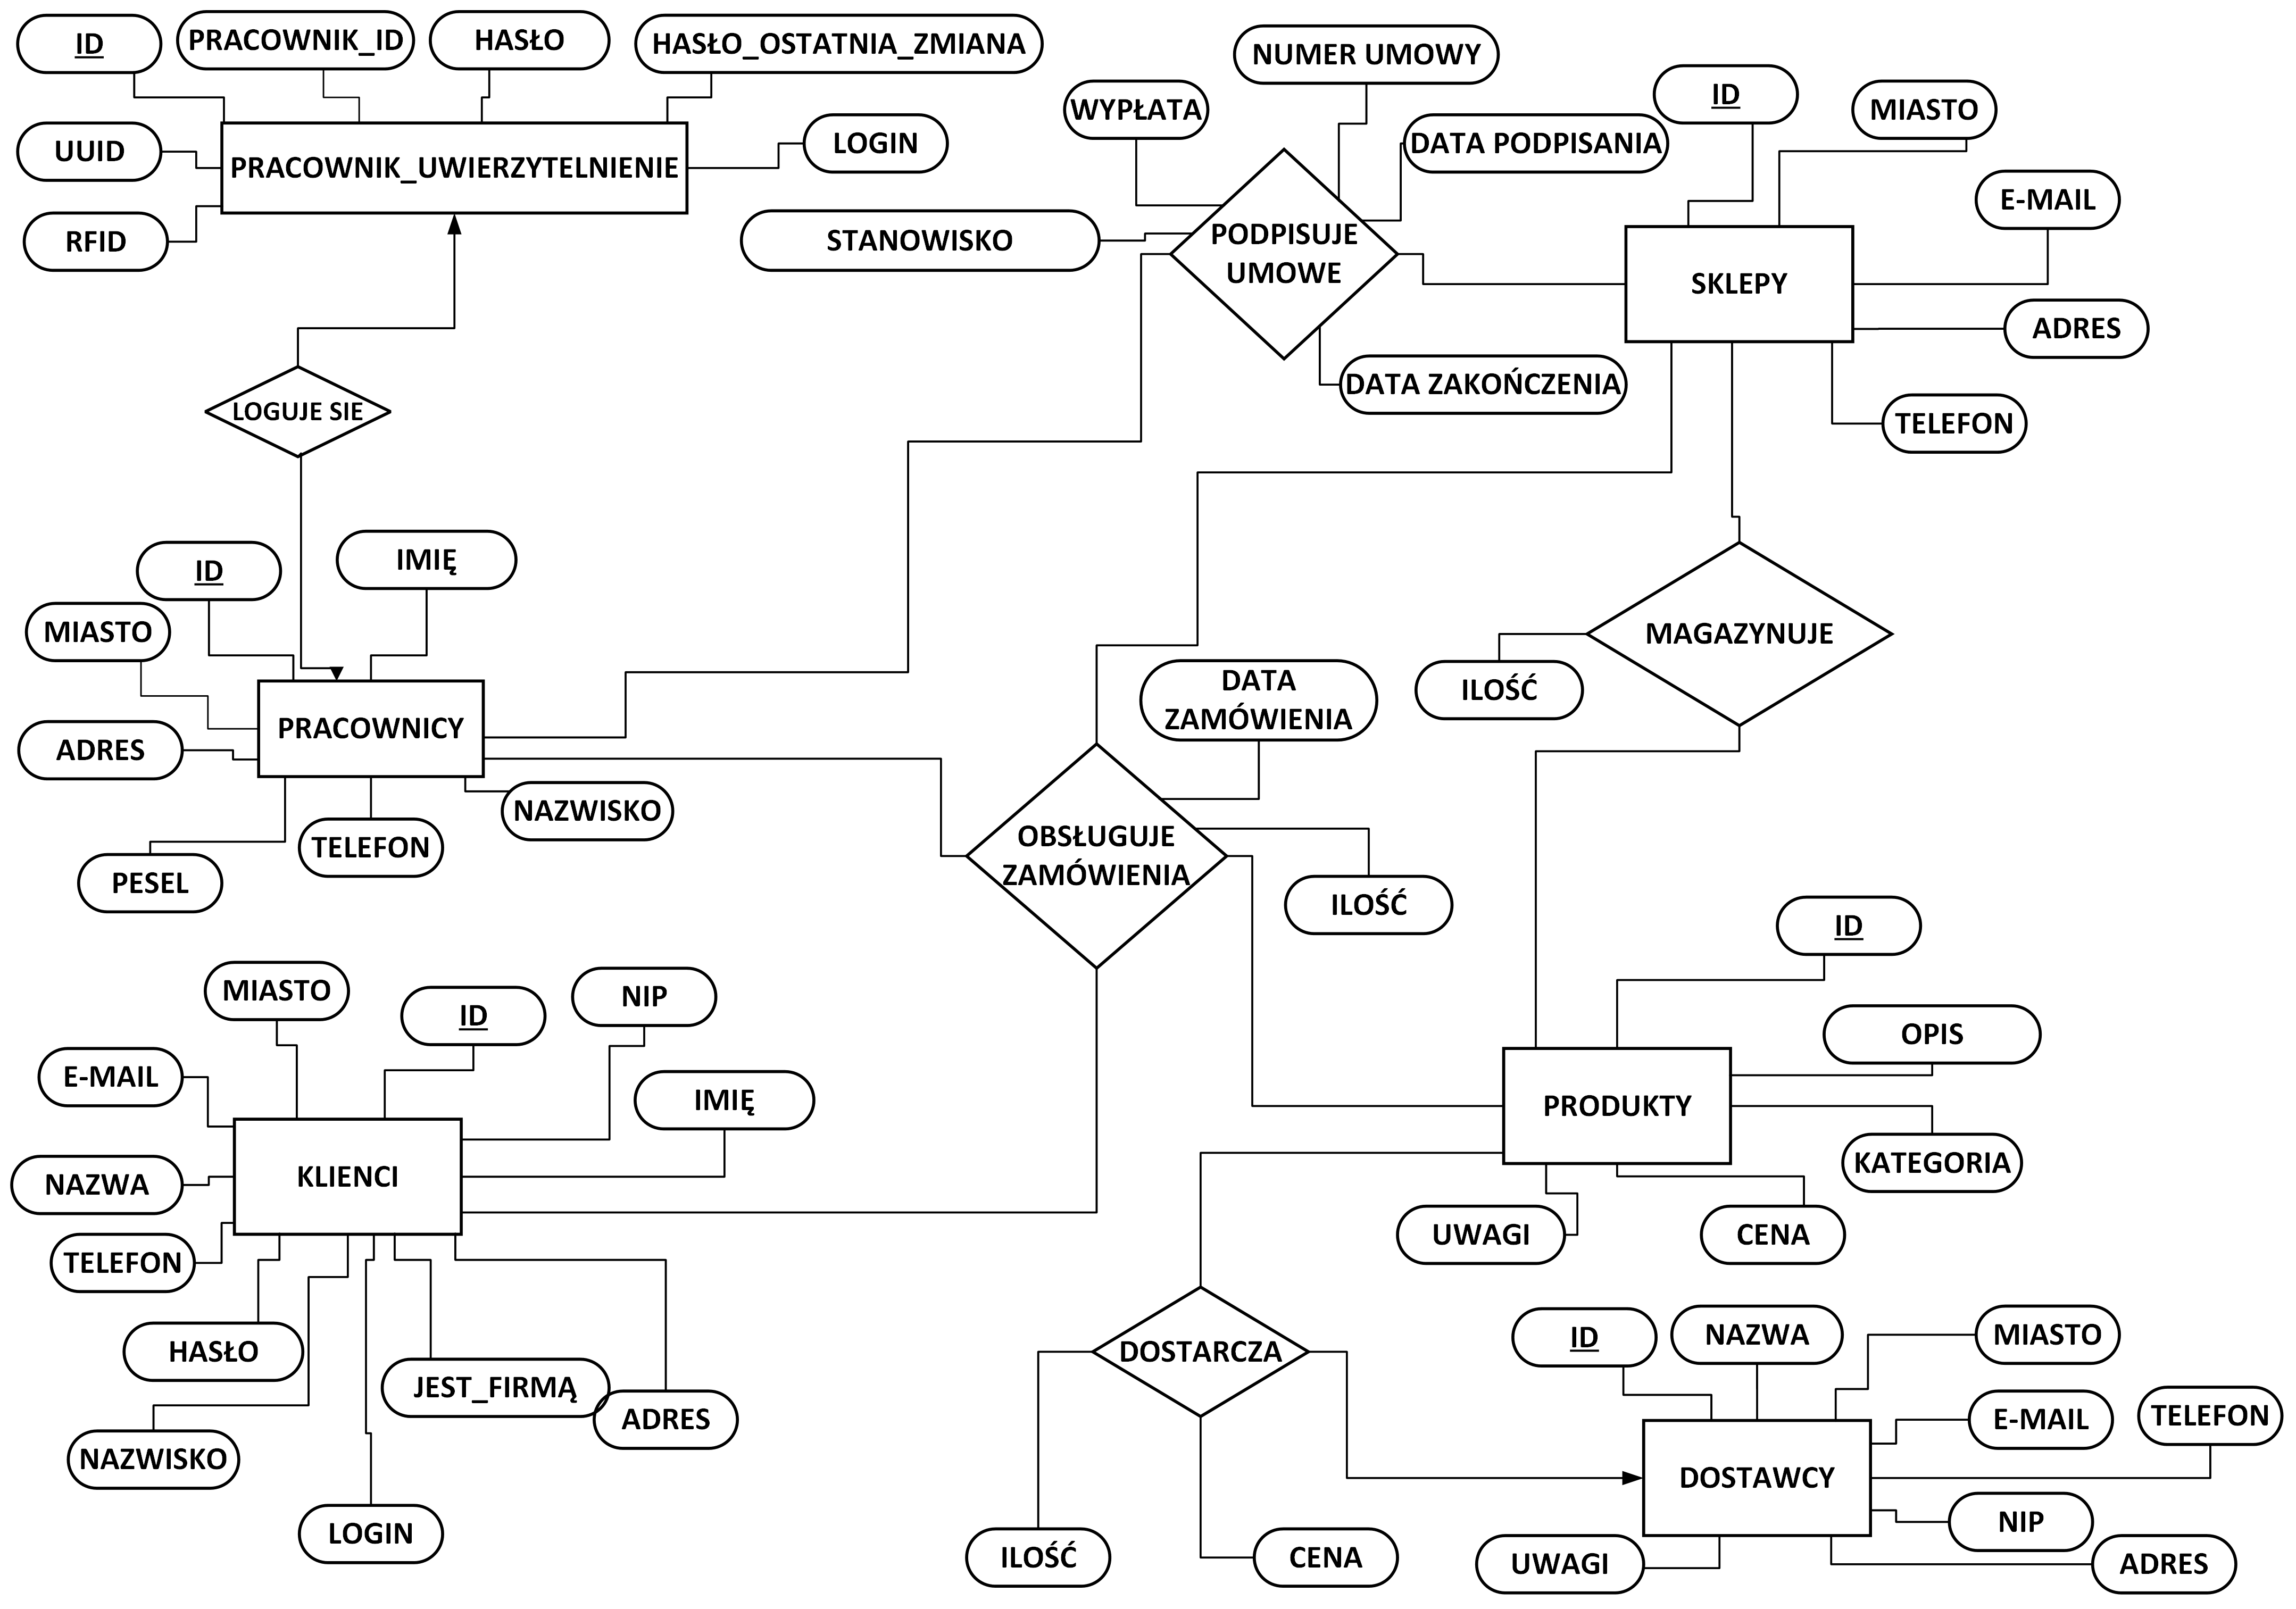
\includegraphics[width=\textwidth]{images/Encja.png}
            \caption{Diagram związków encji}
        \end{figure}
        
    \section{Diagram związków binarnych} 
        \begin{figure}[H]
            \centering
            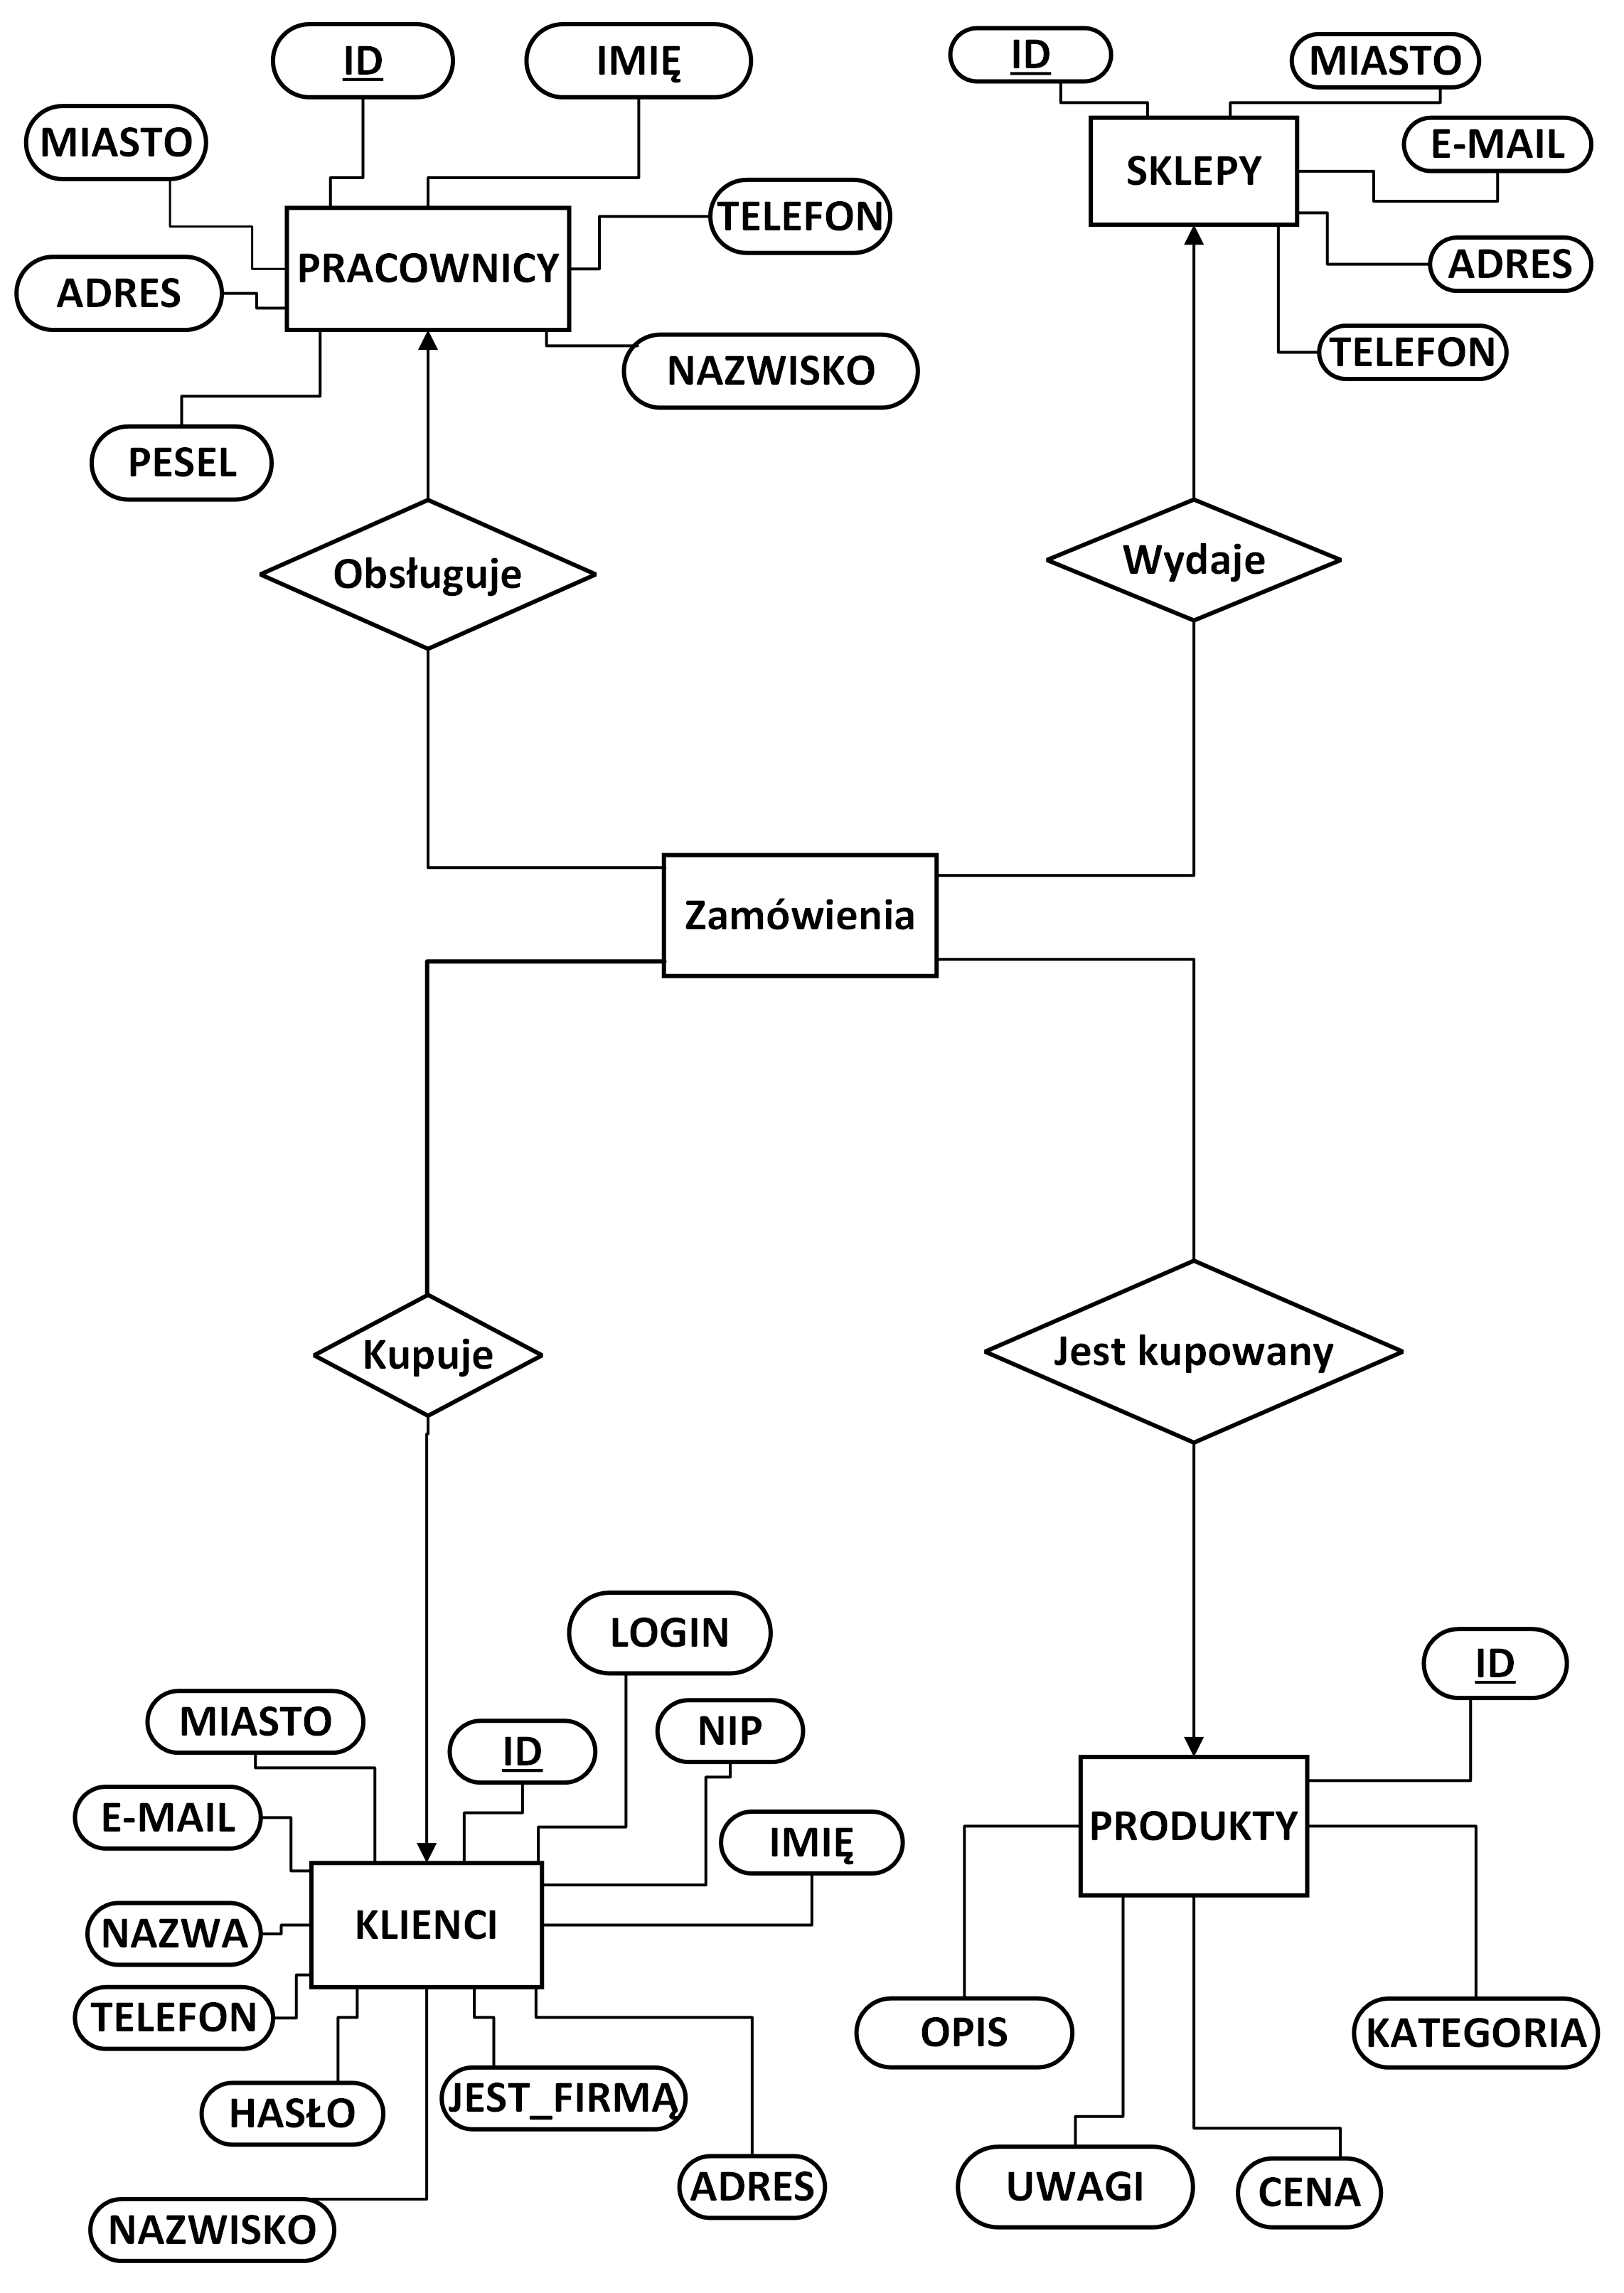
\includegraphics[width=\textwidth, height = 0.88\textheight]{images/ZwiazekBinarny.png}
            \caption{Diagram związków binarnych}
        \end{figure}
        
    \section{Model relacyjny}
        \begin{figure}[H]
            \centering
            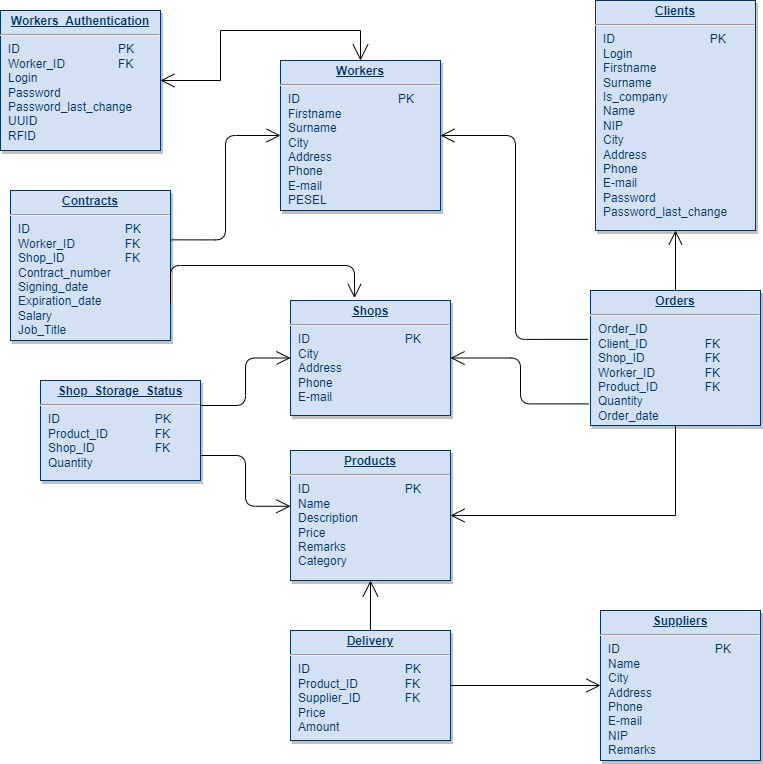
\includegraphics[width=\textwidth, height = 0.88\textheight]{images/ModelRelacyjny.png}
            \caption{Model relacyjny}
        \end{figure}
        
    \section{Wdrożenie}
        \subsection{Aplikacja}
            Aplikacja została wykonana w jęcyku C#, oraz z wykorzystaniem \textit{Windows Presentation Foundation} (WPF) w celu generowania widoku dla klienta. Stworzony panel przedstawia widok na bazę dancyh z poziomu administratora informatycznego. Widzi on wszystkie tabele i zależności.
        
        \subsection{Baza danych}
            Została wykonana z zachowaniem wsyztskich założeń, które zostały dla niej stworzone w tej dokumentacji. Została wypełniona losowymi danymi z wykorzystaniem strony \href{https://www.mockaroo.com/}{mockaroo.com}, która umożliwa generowanie losowych danych w określonych typach, (np. Imię, Nazwisko czy Miasto). Poniżej zamieszamy zrzut ekranu z aplikacji phpMyAdmin prezentujący ostateczny wygląd bazy oraz relacje w niej panujące. W celu zwiększenia użyteczności bazy, stworzono dwa widoki odpowiedzialne za połączenie zamówień z klientami, sklepami, produktami i pracownikami. Drugi widok odpowiada za połączenie produktów z dostawcami, przedstawienie cen zakupu oraz nazw produktów i dostawców, widok ten wyświetlany jest w zakładce produktów oraz dostawców. 
            
            \begin{figure}[H]
                \centering
                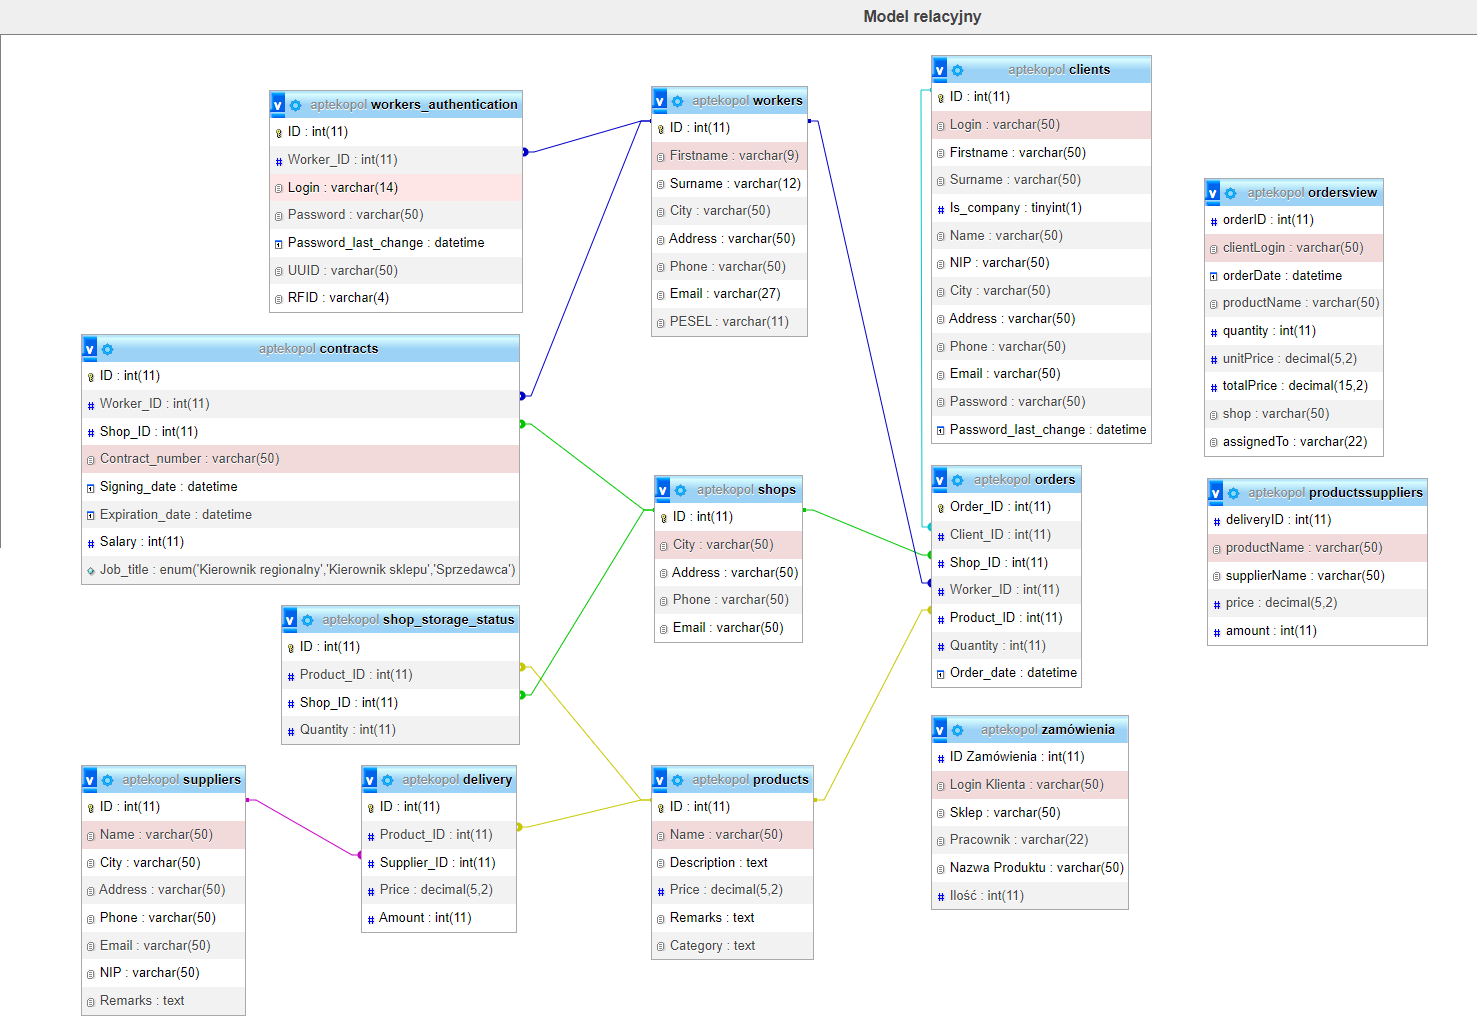
\includegraphics[scale=0.4]{images/phpmyadmin.png}
                \caption{Zrzut ekranu z aplikacji phpMyAdmin, prezentujący model relacyjny}
            \end{figure}
            
        \subsection{Wygląd aplikacji i funckjonalności}
            Stworzona przez nas aplikacja pozwala na zarządzanie pracownikami (edycje, dodawanie oraz usuwanie), zarządzanie sklepami w sieci, zarządzanie produktami oraz podgląd łańcuchów dostaw dla konkretnych produktów, zarządzanie klientami (edycja oraz możliwość podglądu złożonych zamówień) oraz zarządzanie dostawcami (podgląd oraz edycja).
            
            \begin{figure}[H]
                \centering
                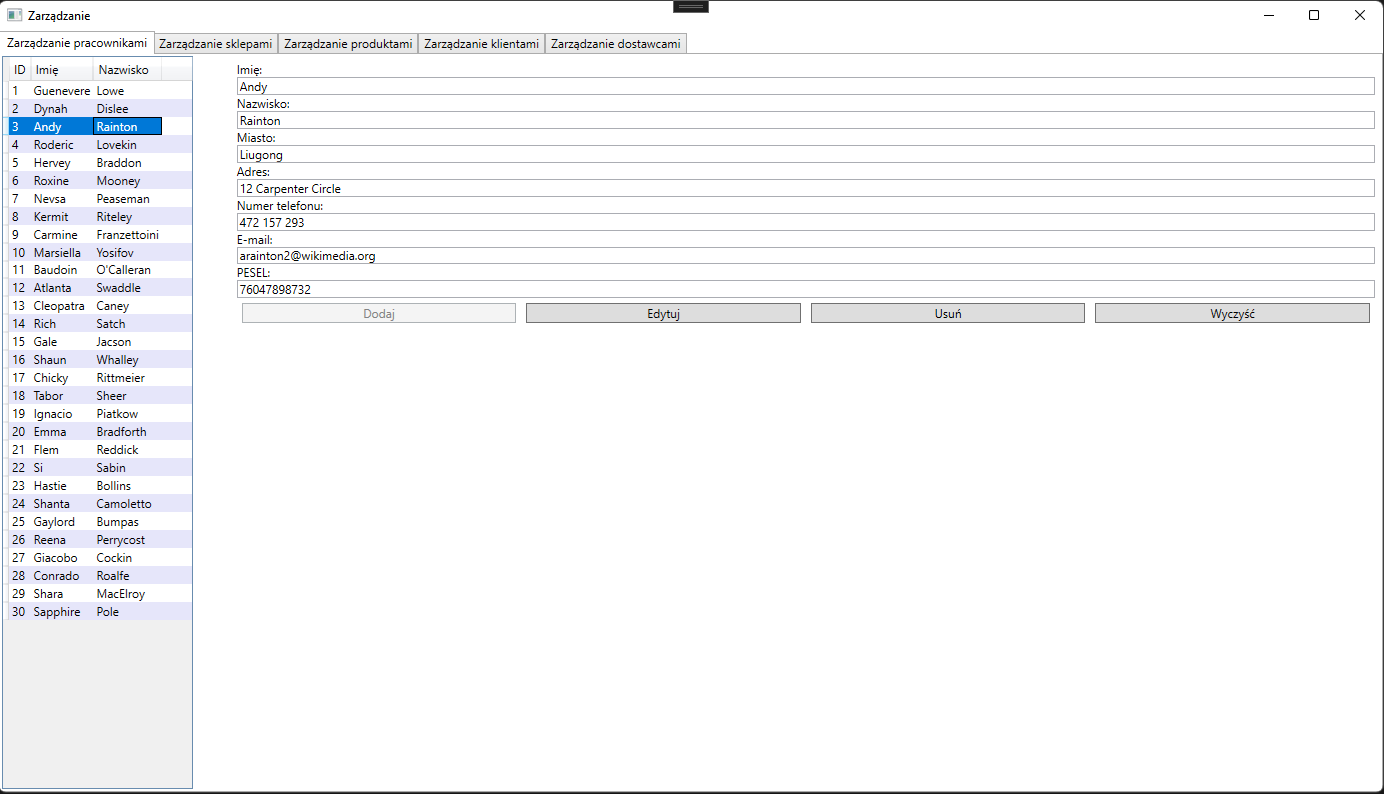
\includegraphics[scale=0.4]{images/pracownicy.png}
                \caption{Zrzut ekranu z aplikacji przedstawiający widok zakładki pracownicy}
            \end{figure}
            
            \begin{figure}[H]
                \centering
                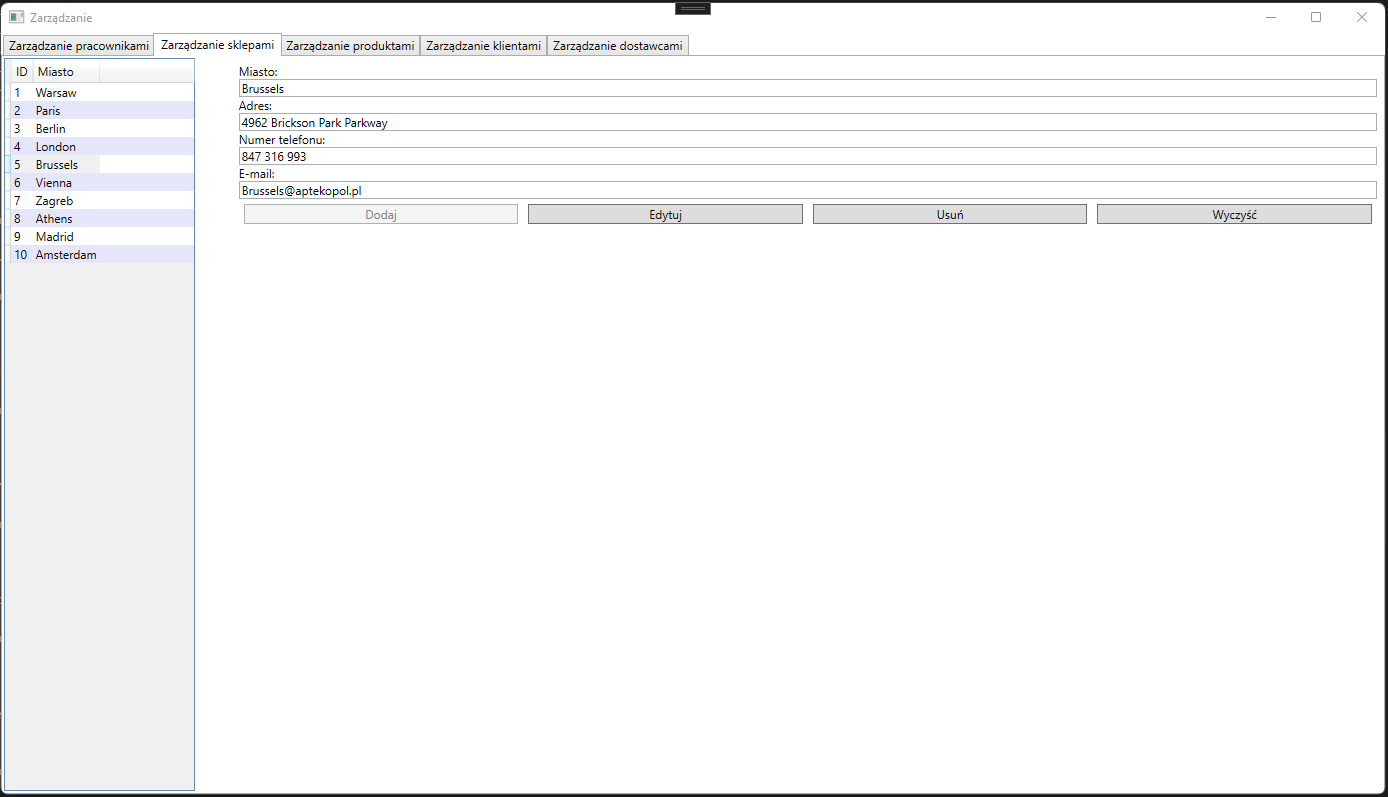
\includegraphics[scale=0.4]{images/sklepy.png}
                \caption{Zrzut ekranu z aplikacji przedstawiający widok zakładki sklepy}
            \end{figure}
            
            \begin{figure}[H]
                \centering
                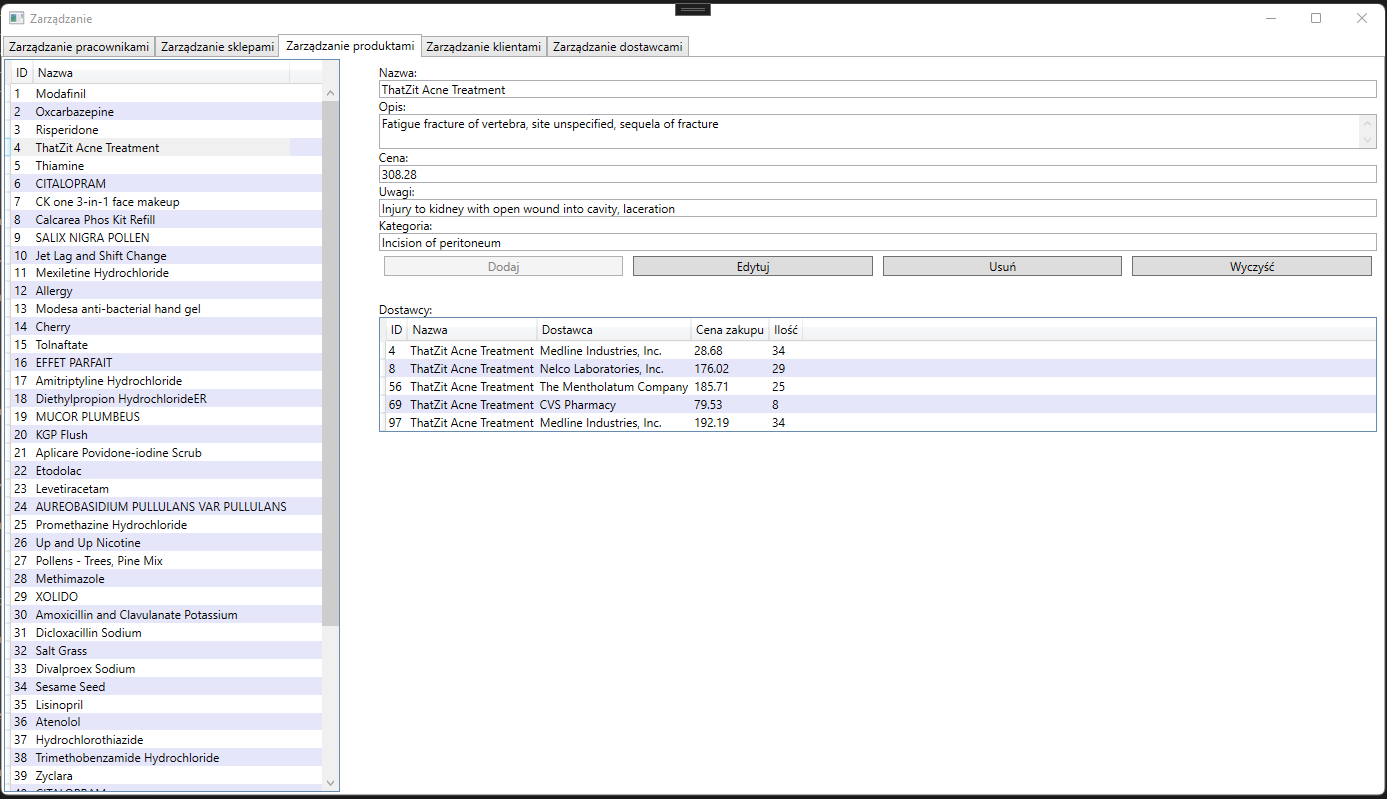
\includegraphics[scale=0.4]{images/produkty.png}
                \caption{Zrzut ekranu z aplikacji przedstawiający widok zakładki produkty}
            \end{figure}
            
            \begin{figure}[H]
                \centering
                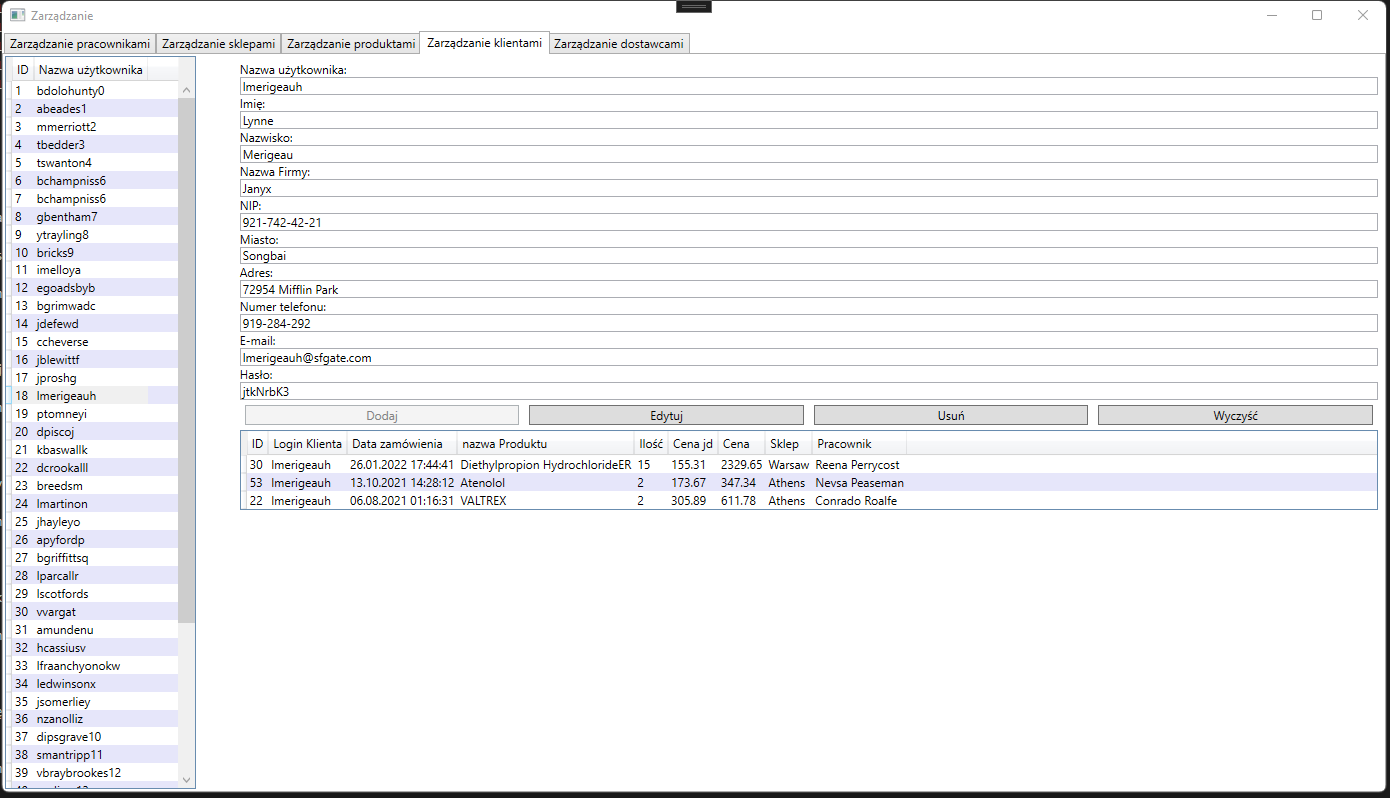
\includegraphics[scale=0.4]{images/kienci.png}
                \caption{Zrzut ekranu z aplikacji przedstawiający widok zakładki klienci}
            \end{figure}
            
            \begin{figure}[H]
                \centering
                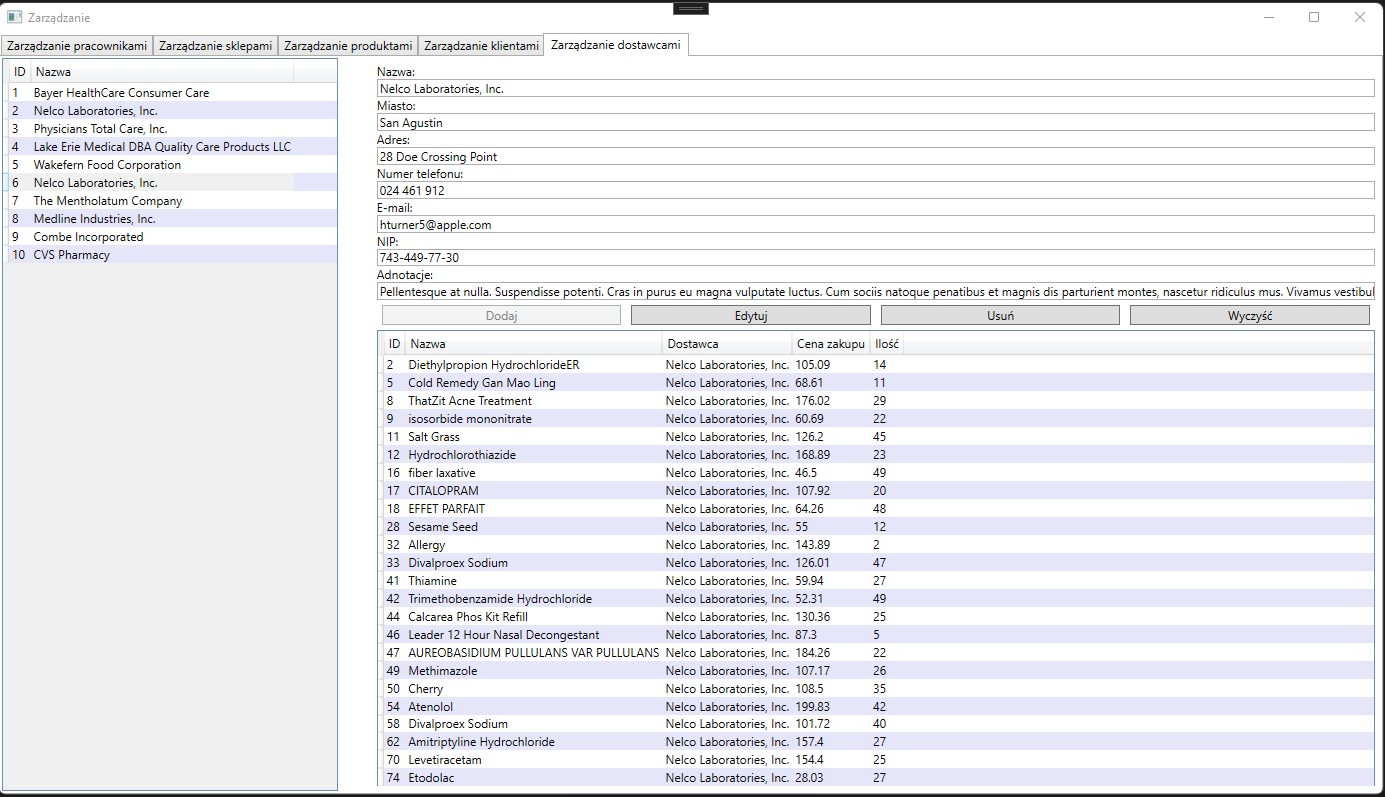
\includegraphics[scale=0.4]{images/dostawy.png}
                \caption{Zrzut ekranu z aplikacji przedstawiający widok zakładki dostawcy}
            \end{figure}
            
            \begin{figure}[H]
                \centering
                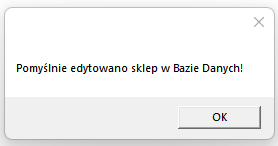
\includegraphics{images/komunikat1.png}
                \caption{Komunikat wyświetlany po poprawnej edycji rekordu}
            \end{figure}
            
            \begin{figure}[H]
                \centering
                
\includegraphics{images/komunikat2.png}
                \caption{Komunikat przy próbie usunięcia rekordu który ma powiązania z innymi, na przykładzie usunięcia sklepu z przypisanymi pracownikami i zamówieniami}
            \end{figure}
            
    \section{Podsumowanie i wnioski}
        \subsection{Podsumowanie projektu}
            Udało się stworzyć bazę danych zgodną z założeniami oraz w pełni funkcjonalną, którą z powodzeniem można użyć w aplikacji do zarządzania małą siecią sklepów. Po testach w aplikacji okazała się być wystarczająca do obsługi podstawowych problemów wystepujących w sklepie.
            
        \subsection{Rozwój}
            Dodanie zdjęć do protuktów, w celu ich szybszej identyfikacji przez klienta i pracownika. Możliwosć sprawdzania obrotów sklepu oraz cąłej sieci, stworzenie tabel odpowiedzialnych za zarządzanie finansami. Dodanie oceny produktów przez klientów i podglądu status zamówienia.
    
\end{document}
